\section{Teorijski okvir}
\label{ch:ch1}

\subsection{Središnja dogma molekularne biologije}

U jednoj stanici organizma nalazi se informacija potrebna za razvoj cjelokupne jedinke. Kod većine organizama ta informacija kodirana je u molekuli koja se naziva deoksiribonukleinska kiselina  (DNK) uz izuzetak nekih organizama koji za tu svrhu koriste ribonukleinsku kiselinu\footnote{Vjerojatno najpoznatiji primjer je HIV virus} (RNK).
Tok genetskih informacija unutar biološkog sustava naziva se središnja dogma molekularne biologije. Slika \ref{fig:dogma} prikazuje analogiju središnje dogme i općeg komunikacijskog modela u računalnoj znanosti. Ribonukleinska kiselina (RNK) je polinukleotidna jednolančana molekula i nastaje transkripcijom komplementarnih baza gena iz molekule DNK. Ovaj se proces odvija pod utjecajem enzima RNK polimeraza koji prepoznaju karakteristično mjesto (promotor) na DNK molekuli gdje započinju proces prepisivanja korištenjem ribonukleotidnih molekula – adenin (A) se prepisuje u uracil (U), timin (T) u adenin, guanin (G) se prepisuje u citozin (C) te obratno, citozin u guanin. Transkripcija se nastavlja dok enzim ne stigne do karakterističnog niza zvanog terminator. Molekula RNK se prenosi iz jezgre stanice u citoplazmu. Na ribosomima u procesu translacije nastaju molekule proteina\cite{Brown01}.
\par
\begin{center}
   \begin{figure}[ht!]
      \begin{center}
         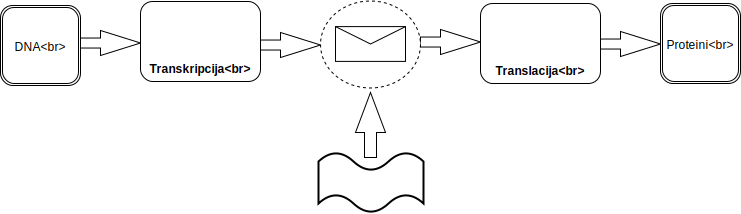
\includegraphics[height=5cm, width=14cm]{central_dogma}
                 \caption[Središnja dogma molekularne biologije]{\textbf{Središnja dogma molekularne biologije prikazana kroz dijagram općeg komunikacijskog sustava prema Shannonu\cite{Shannon01}.} \textit{DNK molekula je izvor informacije, a poruka sadrži uputu za sintezu proteina. Odašiljanje poruke je transkripcijski proces koji kodira poruku. Signal se prenosi prema prijemniku, ribosomima u obliku RNK molekule. U procesu translacije dekodira se poruka i nastaje molekula proteina. Šum označava greške u internim biološkim funkcijama stanice, ali i vanjske utjecaje koji mogu utjecati na ovaj proces.}}
         \label{fig:dogma}
      \end{center}
   \end{figure}
\end{center}

\subsection{Izrezivanje RNK molekule}
Elektronskim mikroskopom utvrđena je mozaična struktura gena (Slika \ref{fig:intron}). Ovo je potvrđeno u eksperimentima zonskog centrifugiranja gdje je ustanovljena razlika sedimentacije primarnih transkripata i zrelih mRNK molekula \cite{Berg01}.
\begin{center}
   \begin{figure}[ht!]
      \begin{center}
         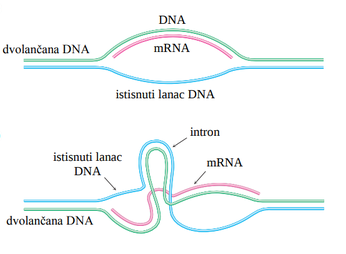
\includegraphics[height=6cm, width=8cm]{introni}
                 \caption[Detekcija introna elektronskim mikroskopom]{\textbf{Detekcija introna elektronskim mikroskopom.} \textit{Kod kontinuiranih gena vidi se samo jedna omča dvolančane DNK (gore). Ako gen sadržava introne, vide se dvije omče jednolančane DNK i omča dvolančane DNK (dolje). Crvenom bojom prikazana je mRNK. Preuzeto iz \cite{Berg01}.}}
         \label{fig:intron}
      \end{center}
   \end{figure}
\end{center}
Jednu DNK molekulu čini više različitih gena između koji se nalazi niz nekodirajućih nukleotidnih baza. Unutar većine gena\footnote{kod eukariotskih organizama} nalaze se intervencijske sekvence (Slika \ref{fig:gene}). DNK se transkripcijom prepisuje u primarni transkript RNK. Intervencijske sekvence nazivaju se introni i oni ne kodiraju proteine nego se izrezuju iz primarnog transkripta. Zrela mRNK (engl. \textit{messenger RNA}) molekula sastoji se samo od kodirajajućih dijelova nazvanih egzoni.
Granica između egzona i introna naziva se donorsko mjesto (EI), a granica između introna i egzona akceptorsko mjesto (IE). Mehanizam obrade primarnog transkripta u kojem se izbacuju nekodirajući te spajaju kodirajući slijedovi baznih parova naziva se izrezivanje ili prekrajanje (engl. \textit{splice}). Detalji ovog mehanizma nadilaze opseg ovog rada i detaljno su opisani u \cite{Brown01, Cox01}. Međutim, jasna je motivacija za pronalaskom algoritma koji može detektirati ove lokacije u genu. Kada se sekvencira novi genom ili pronađe novi protein za koji nije poznat gen koji ga kodira ovakav algoritam može detektirati potencijalne kandidate i uvelike suziti izbor između milijuna, odnosno milijardi potencijalnih pozicija u genomu.
\begin{center}
   \begin{figure}[t!]
      \begin{center}
         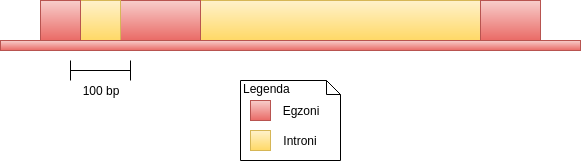
\includegraphics[height=4cm, width=14cm]{intron_egzon}
                 \caption[Introni]{\textbf{Introni.} \textit{Struktura ljudskog $\beta$-globin gena. Ovaj gen dug je 1423 bazna para (bp) i sadrži dva intron, prvi dužine 131 bp i drugi dužine 851 bp što čini oko 69\% dužine gena. Prilagođeno prema \cite{Brown01}.}}
         \label{fig:gene}
      \end{center}
   \end{figure}
\end{center}
